\documentclass[12pt]{article}
\usepackage[margin = 1 in]{geometry}
\usepackage{amsmath, amsfonts, graphicx, amsthm}

\newcommand{\F}{\mathbf{F}}
\newcommand{\C}{\mathbb{C}}
\newcommand{\R}{\mathbb{R}}
\renewcommand{\P}{\mathbb{P}}

\newtheorem{fact}{Fact}
\newtheorem{definition}{Definition}

\title{Algebraic Geometry Notes}
\author{Raman Aliakseyeu}
\date{Winter 2024}

\begin{document}
    \maketitle
    We will start with projective geometry, and then add algebra to it. No schemes in this course, we will be closer to the 19th century stuff. We are not following any particular book(s). Number one book is "Algebraic Geometry" by Shafarevich, our goal is all of chapter 1. We will start with projective geometry, a book for that is (on canvas). 
    \section{Projective Geometry} % TODO: title this unit
    \subsection{Lecture 1} % TODO: name the lectures
        Algebraic geometry studies solutions to systems of algebraic equations/algebraic curves (which are loci of solutions of algebraic equations). One of the most famous renaissance geometry results is the Pascal theorem: the points $G, H, I$ in the diagram below are colinear for any configuration of $A, B, C, D, E, F$ on the circle. 
        \begin{center}
            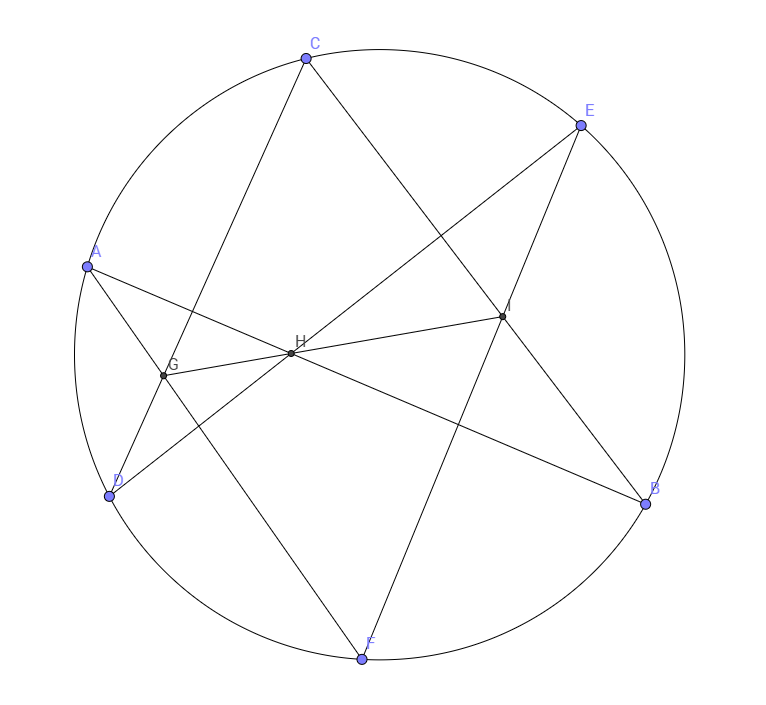
\includegraphics[width = 0.5 \linewidth]{pascals-theorem.PNG}
        \end{center}
        A similar result to that is Pappus' theorem. Another top theorem is by Cayley-Salman 1849: A smooth projective cubic surface contains exactly 27 lines. Another such theorem is that any smooth projective curve of degree 4 has 28 bitangent lines (tangent in exactly two points). Working toward proofs of these results using algebraic geometry is our goal. \par 
        \textit{History of the subject}: throughout the 19th century it developed very quickly, people who were into Euclidean geometry just transitioned to algebraic geometry and discover miracles like we described above. During the late 19th century Italians, who before led algebraic geometry, started producing very incorrect results because the technical aspects became too hard. Oscar Zariski and others saved the subject by rigorizing it using commutative algebra, with the language of ideals and rings, etc. We will see some `wrong' arguments by the Italian school and see why they are not precise enough. There was another revolution by Grothendieck and the Bourbaki group in developing the language of schemes, which we will not touch in this course (``You will need to sacrifice a year of your life to start speaking that language. I never needed to, but a lot of people do.'')\par 
        (Rudenko plug: woollymathematics.com)\par 
        Take $\F$ to be some field (usually $\C$), and polynomials $p_1, \dots, p_k \in \F[x_1, \dots, x_n]$, and study the solutions to the system 
        $$\begin{cases}
            p_1(x_1, \dots, x_n) = 0 \\
            \vdots \\
            p_k(x_1, \dots, x_n) = 0
        \end{cases}$$
        \begin{fact}
            If $k = 1$ and $p_1(x) = x^d + a_{d-1}x^{d-1} + \dots + a_0$ for $d \geq 1$, $p_1(x) = 0$ has $\leq d$ solutions in $\F$. 
        \end{fact}
        If $k = 2$, the number of solutions is $\leq$ than the product of the degrees of the polynomials. Of course we usually want a precise number of solutions, but generally we can't hope for anything more than upper bounds. 
        \begin{fact}
            If $\F = \C$, then $p(x) = 0$ has a solution. 
        \end{fact}
        This is a remarkably hard result called the Fundamental Theorem of Algebra. There is a result that is in a way easier:
        \begin{fact}
            If $\F = \C$, then $p(x) = 0$ has exactly $d$ solutions if counted with multiplicity. 
        \end{fact} 
        We would hope for something like that but for $k > 1$. Bezoiut's theorem kind of satisfies that, but the picture is more complicated. For example, take a line and a hyperbola. While we would expect $4$ solutions up to multiplicity, but take a line intersecting one of the components of the hyperbola transversally that is parallel to one of the other component's asymptotes. However, everything becomes nicer if we change the complex plane to the projective plane. The study of geometry on the projective plane is the projective geometry, and that's what we will study first. \par 
        \begin{definition} \label{def:proj_plane}
            Let $\F$ be a field. A \textbf{projective space} $\P_\F^n$ is the set of lines in the vector space $\F^{n+1}$. 
        \end{definition}
        An example for $\F = \R$, $\P_{\R}^2$ is the set of lines through the origin in the real plane. We can think of $\P_\R^1$ as all the points of a line in $\R^2$ not through the origin (say the line $y = 1$ in $\R^2$) but with a point at infinity added. \par 
        In $\R^2$, usually two lines intersect at one point, and two points are contained in one line. We can also define $\P_\R^2$ as the set of points of $\R^2$, and the set $[l]$ (points at $\infty$), which are equivalence classes of lines in $\R^2$ by $l_1 \sim l_2$ for $l_1$ and $l_2$ are parallel. Note that there is one more line, line at infinity, consisting only of points $[l]$. \par 
        \begin{fact}
            In $\P^2_\R$ every two distinct lines intersect in one point and every two points are contained in precisely one line. 
        \end{fact}
        \begin{proof}
            Non-parallel lines intersect in the usual way. Parallel lines intersect at their equivalence class $[l]$. If one of the lines is the `line at infinity', they intersect at the equivalence class of the other line. Similarly we can examine the second part of the statement. 
        \end{proof}
        \begin{fact}
            For $\P_\R^2$, the abstract definition \ref{def:proj_plane} is equivalent to the definition we gave in the example. 
        \end{fact}
        \begin{proof}
            Take a plane in $\R^3$ not passing through the origin, $z = -1$ for example. Then we can create a bijection between the set of lines through the origin and the set of points on the plane and the set of points at infinity, by mapping the lines that intersect the plane with their intersection point, and those that are parallel with the plane to their equivalence class on the plane $\R^2$. Thus we have a bijection between the two objects we defined. 
            \begin{center}
                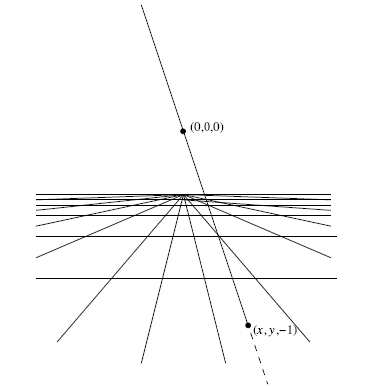
\includegraphics[width = 0.4\linewidth]{proj-plane.jpg}
            \end{center}
        \end{proof}
        Another way to think of $\P_\R^2$ is as a sphere with antipodal points identified. \par
        ``ChatGPT can make you Snake 4: Snake but on the projective plane.''
    
\end{document} 